\chapter{Background} \label{ch:[chapter 2 label]}

In this section, I discuss important background for setting the context of my research. This includes brief details about cognitive processes, like formulating \gls{information_need}s, resulting user search behaviors, and how a search system technically attempts to interpret user requests. To give an overview of the IR process, figure \ref{fig:Background_Complete_Search_System}. depicts the components of a complete search system. The IR  process is both cognitively and technically complex, therefore I have summarized important steps for my research in figure \ref{fig:Background_IR_Steps}. IR is a very large field and a deeper discussion is outside the scope of this proposal. However, I leverage many fundamental research techniques from the IR community, so I refer readers to comprehensive IR literature on user needs and interactions while searching \cite{White2016}, modern IR system architectures \cite{Baeza-Yates1999}, and IR data structures and algorithms including the vector space model and relevance feedback \cite{Buckley1985}.

\begin{figure}
    \centering
    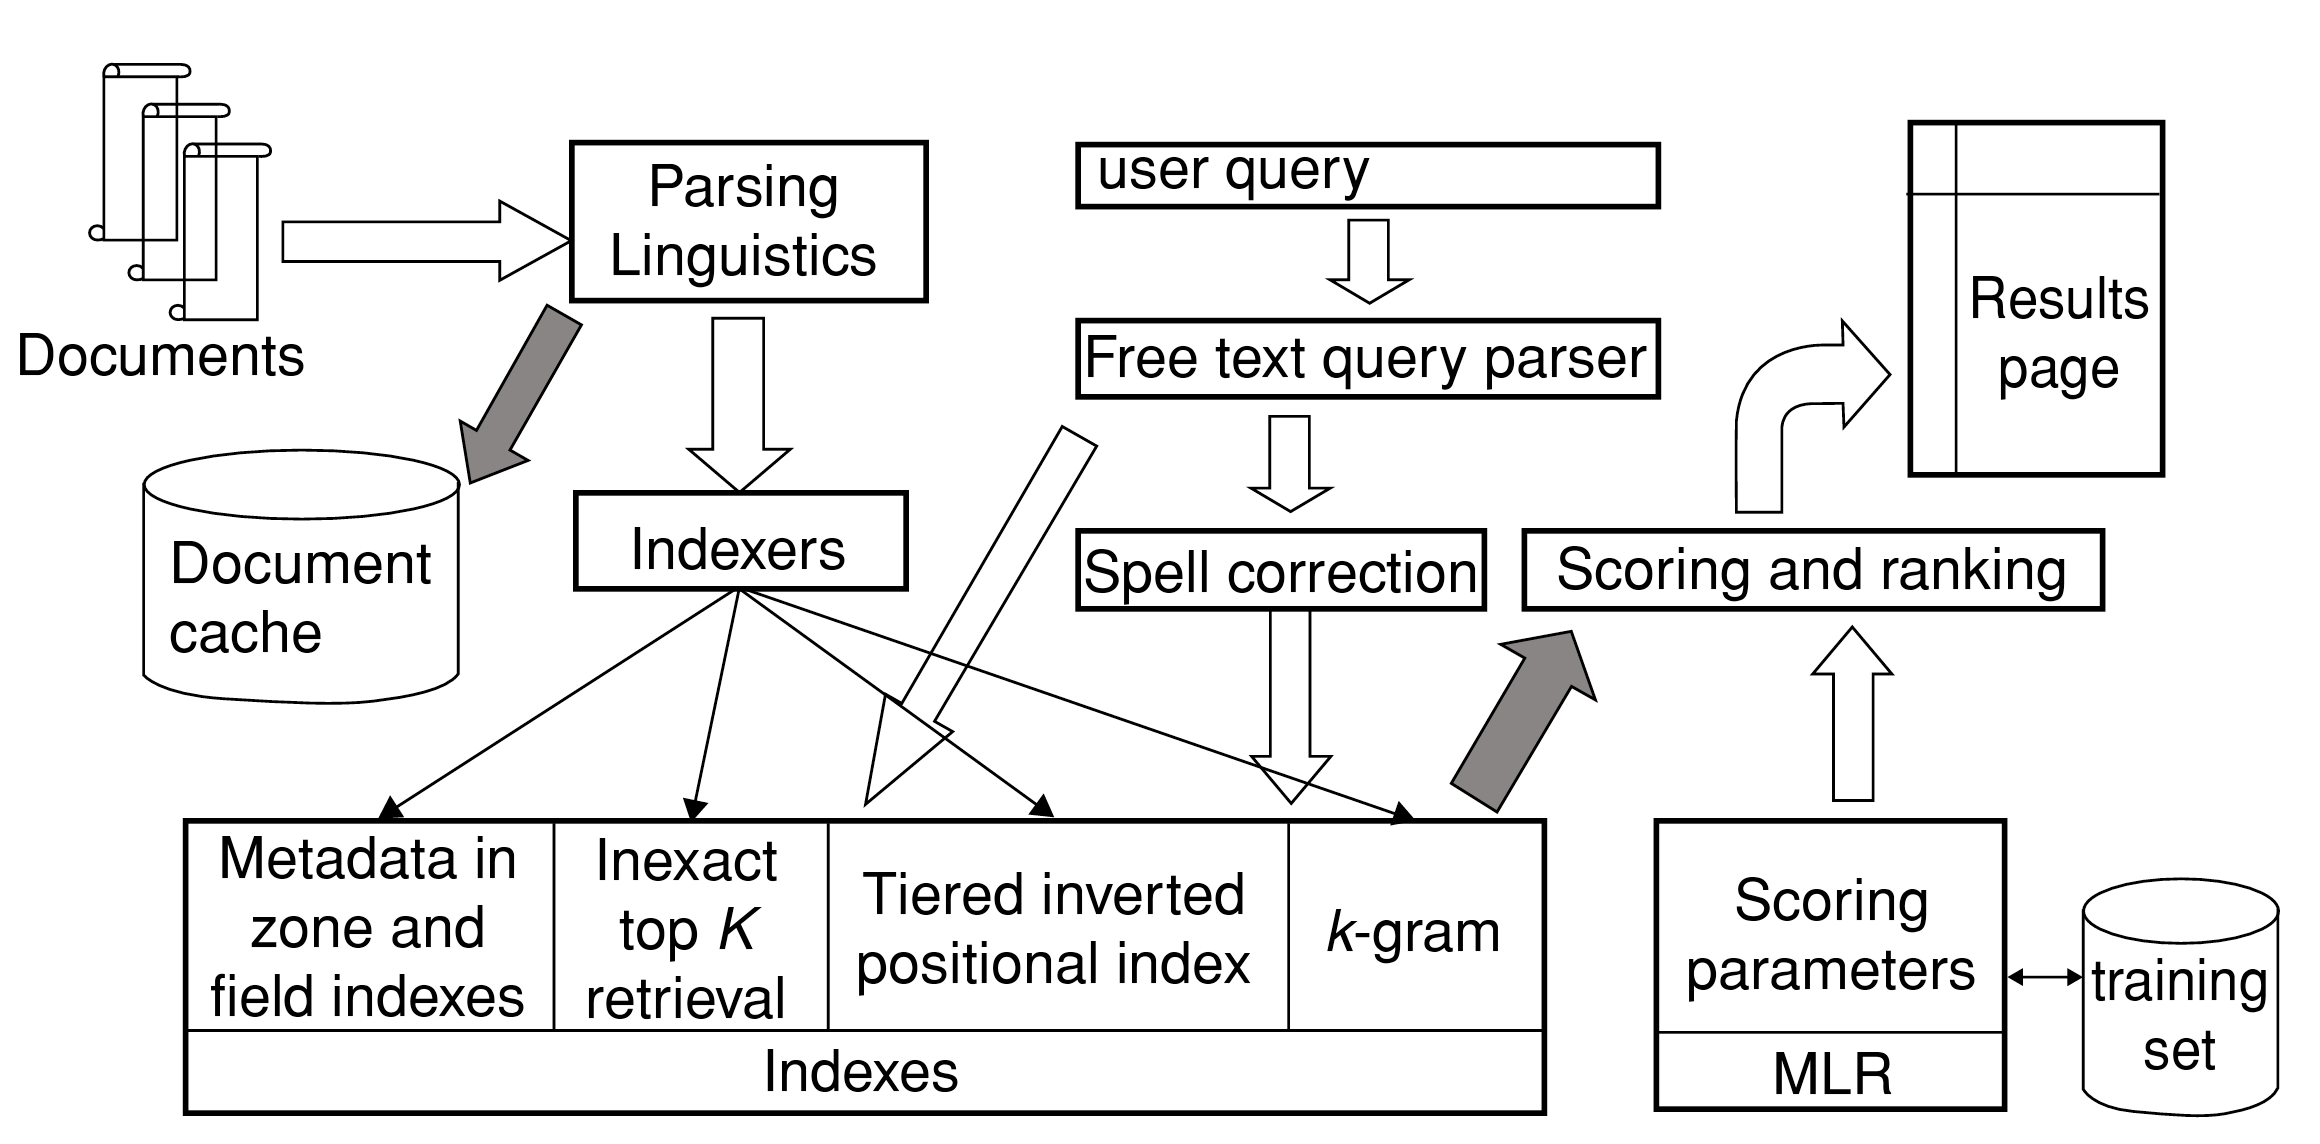
\includegraphics[width=1\textwidth]{../figures/Background_Complete_Search_System.png}
    \caption{This figure, borrowed from \cite{Manning2008}, depicts a complete search system. On the left side of the figure, documents are parsed an indexed to be retrieved. In the center, a user’s query is ingested and parsed. On the right, scoring parameters are used to compare a parsed query and indexed document representations. Documents are assigned a final composite score calculated by linearly combining similarity scores between documents and a query for multiple criteria. The output is a ranked list of results on a page typically called a search engine results page (SERP).}
    \label{fig:Background_Complete_Search_System}
\end{figure}

\begin{figure}
    \centering
    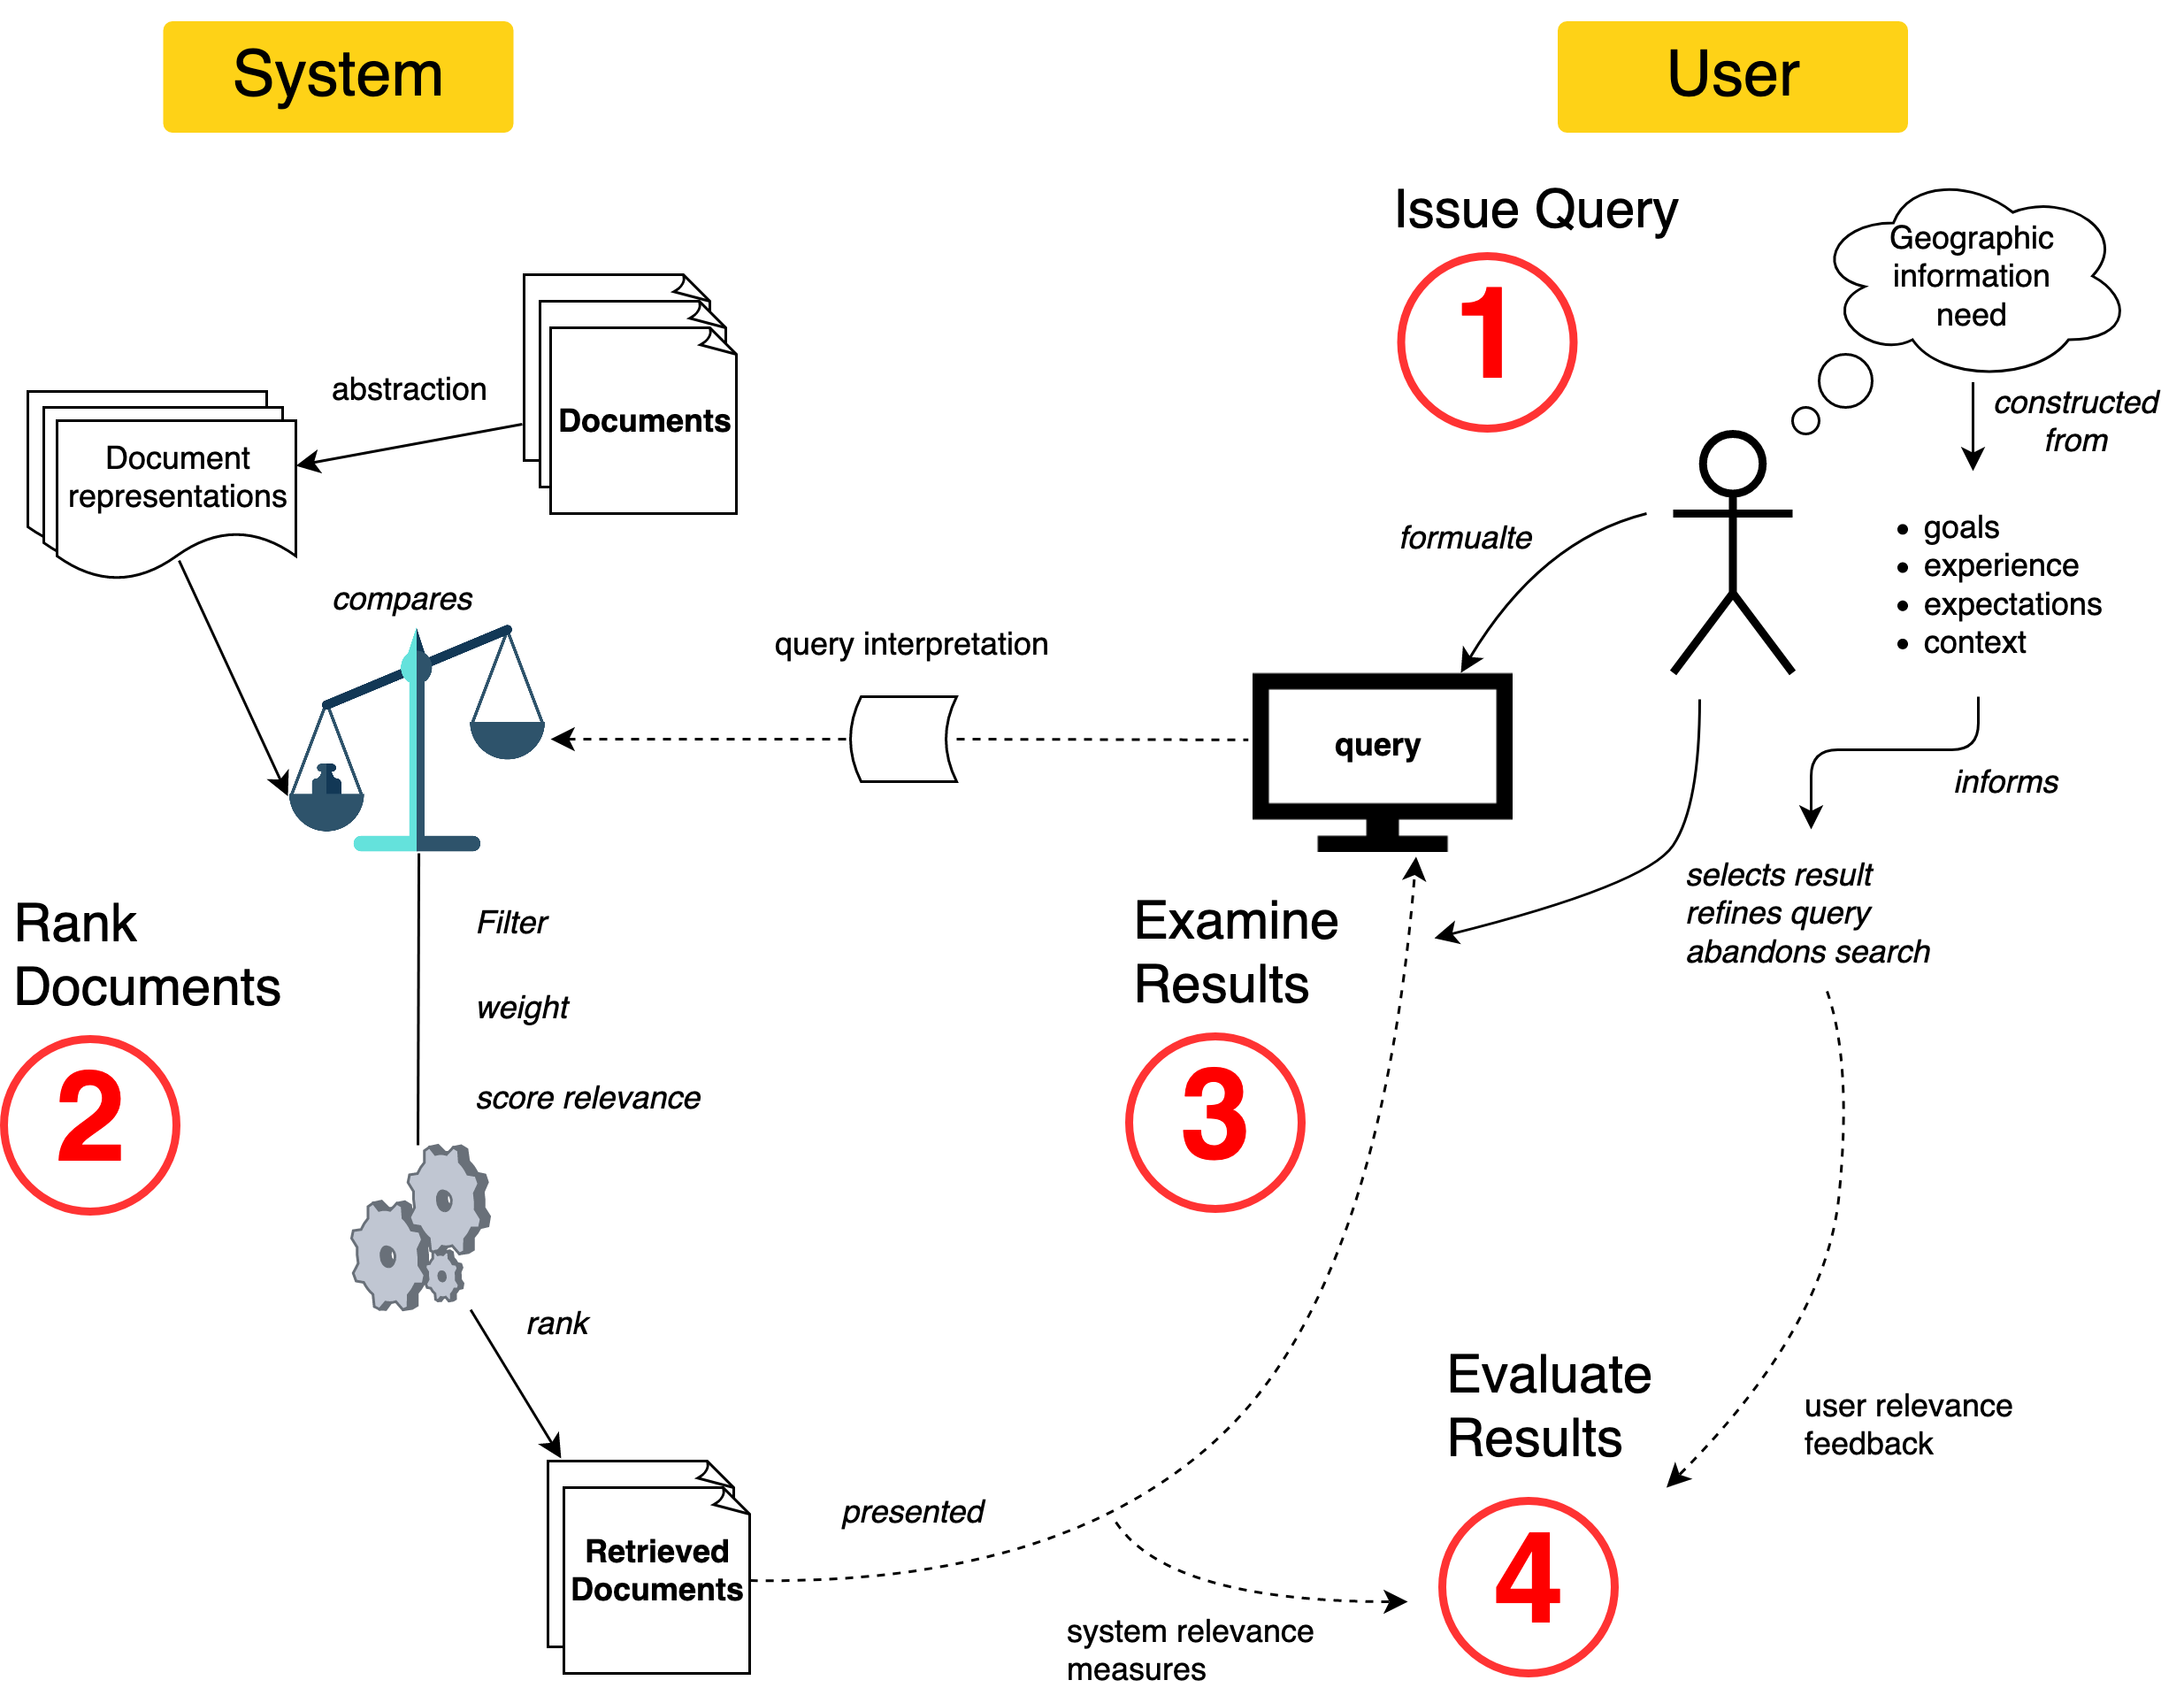
\includegraphics[width=1\textwidth]{../figures/Background_IR_Steps.png}
    \caption{A simplified overview of the IR process with emphasis on steps important to this study. Dashed lines represent information transfers and italics represent actions. Step 1: User formulates and issues a query based on GINs. Step 2: Search system compares document representations and a query interpretation and ranks documents by relevance. Step 3: Resulting documents are ordered, presented, and examined by the user. Users then select and explore results, refine their query, or abandon search. Step 4: A system is evaluated for effectiveness based on user relevance feedback and/or system relevance measures including precision, recall, MAP, and NGDC, among others. See glossary for measure definitions.}
    \label{fig:Background_IR_Steps}
\end{figure}

\section{Geographic Information Needs of Data Searchers}

Users who search for data have needs that are diverse, uncertain, and sometimes hard to describe. Ultimately, users have diverse questions that produce diverse needs that in turn guide \gls{information_seeking} activities. Some users have a targeted goal that they need to accomplish, like finding a dataset on crime or navigating to the nearest bus station. We call this information seeking activity searching because it is active and directed. Other users' needs are more relaxed. They explore what is available out of curiosity or in hopes of discovering something new and useful. We call this information seeking activity browsing. Users articulate their needs in diverse ways as well. In text-based search, some users express their needs using natural language while others use keywords or topics. What is more, diverse needs yield even more diverse expectations. For example, users that perform a targeted search are typically seeking a specific type of information, but how that information is labeled, how it is presented, and its required contents are just a few expectations that a user could have. Broadly speaking, the domain of IR studies these needs along with the "representation, storage, organization of, and access to information items such as documents, Web pages, online catalogs, structured and semi-structured records, [and] multimedia objects" \cite{Baeza-Yates1999}. The authors of this book on modern IR also highlight how, "the representation and organization of the information items should be such as to provide the user with easy access to information of their interest" \cite{Baeza-Yates1999}. In other words, IR attempts to structure and serve relevant resources to a user based on their articulated needs. And ultimately, a user is looking for information objects that have maximal utility for these needs.

Since user needs are often abstract or complex, they can rarely be directly observed except by asking users what they need. This approach is both unreliable and impractical. So, the IR community instead studies user needs indirectly by observing user search behavior and asking users for feedback. The theory is that someone who is engaged in an information seeking activity will give clues to their needs based on what they search for and how they search for it. These clues act as traces of their behavior. For example, if someone searches for "tacos near me" on the Yelp platform at noon, it can be inferred that they want to find a place for lunch that serves tacos, and to accomplish this, they need information about restaurants. To a human this query is easy to understand. However, for computers this is a monumental task. IR systems must try to comprehend human language as humans do. However, what is important to users remains unclear in the first place. There is an ongoing debate about how concepts like \emph{relevance}, \emph{usefulness}, and \emph{satisfaction} are related, which is preferable to study, and how to evaluate them. Since IR systems cannot directly interpret user needs, they should try to interpret the next closest things, relevance, usefulness, and satisfaction. In the related work section I will discuss these three terms in detail, but first I will discuss user search behavior–primary data for IR research.

\section{User Search Behavior}

Recording user search behavior is a critical step towards understanding user needs. Much like observing people in a psychological study, observing how a user interacts with a search system provides many clues as to what they want to do, what they ended up doing, and what the system should do to be more effective. Search behavior is in essence what users do when the search. This includes practically everything from what they search for to how long it takes for them to get stuck to how often they give up. Search behavior is studied because relevance, usefulness, and satisfaction inferences can be made from particular behaviors. For example, broadly speaking, if a person uses a search tool and exits quickly or continually refines their search queries, they haven't found an \gls{information_object} (\acrshort{IO}) to satisfy their needs. If they dwell on a result for a long time, it can be assumed that they are interested in that result. Once behavior is understood, researchers can change a search system and then record the difference in behavior. For example, if changing a ranking algorithm rearranges the top ten results, researchers can study if users have a strong positional bias and pick the top results, or if they're still drawn to a result that was picked before, indicating that both the result is relevant and that modifying the order doesn't affect behavior.

Studying search behavior is not an easy task since there are many factors that can influence and bias a user. For example, on a search result page (typically called a \acrshort{SERP}) the positionality, authority, and visual appeal of results can attract users to certain results \cite{Hofmann2016}. There are also contextual factors that are hard to control for, such as a user's prior knowledge, their search environment, and their cognitive bias (i.e., favoring positive-sounding search results) \cite{Hofmann2016}. However, some broad behavior patterns have emerged and many specific ones are under investigation. First, most users are somewhat impatient and use search tools for very little time. If they do not find an answer in a short period of time, they will refine and execute their query . After a few executions, many will abandon the search session and seek information elsewhere. Second, users quickly navigate results. Many studies of query logs, system records such as queries, clicks, and transactions, show that users will click on a result, return to the SERP, click on another result, return to the SERP, click on the first result again, etc. To a human, this pattern indicates that a user is comparing results, but to computers this behavior is often difficult to process. Third, the use of query keywords follows the power law. Most query logs show that the same queries and query keywords are issued over and over with a very long tail of infrequent queries. This is important because a search system should make sure that it correctly handles the bulk of queries, especially if they're repeated, but also do not neglect the diverse needs of users. These patterns are just a sample of user expectations, progressions, and articulations.

There are no research approaches that can completely control for individual search behaviors. Furthermore, the relationship strength between someone's information needs and their search behavior is subject to debate. Fortunately, studies over the last few decades have used search behavior patterns to produce a set of robust methods for system-oriented testing and evaluation. That is, there are quantitative methods for testing a systems effectiveness at retrieving relevant documents. The Cranfield approach has become a foundation for modern IR \cite{Sanderson2010}. In this approach, a controlled set of test queries, test documents, and relevance judgements are used to simulate users interacting with an IR system. Test data are benchmark collections created at conferences and working groups like the annual Text Retrieval Conference\footnote{\url{https://trec.nist.gov/}} (\acrshort{TREC}). Researchers change system components, like document indexing and relevance ranking, and evaluate if the changes are an improvement or not \cite{McGill1979}. This approach uses common outcome-oriented evaluation measures to evaluate a system's effectiveness including \emph{\gls{precision}} (i.e., the percentage of selected results that are relevant), \emph{\gls{recall}} (i.e., the percentage of relevant results that are selected), \emph{\gls{mean_average_precision}} (\acrshort{mean_average_precision}) (i.e., precision across multiple queries), \emph{\gls{normalized_discounted_cumulative_gain}} (\acrshort{NDCG}) (i.e., graded relevance of a document based on its rank position), and other quantitative metrics. Human searchers, their behavior, and their interpretations are ignored.

Recently, there has been a rising interest in user-oriented testing and evaluation. As opposed to the system-oriented perspective, the user-oriented perspective tries to achieve a higher level of realism. This means that there is a higher focus on what users want out of a system, what results they find useful, and what ultimately satisfies them, not just how good a system is at retrieving the right results based on predefined relevance rules. This approach evaluates a system using process-oriented evaluation measures. This means that it attempts to evaluate how a user feels during the search process based on behavior and user feedback. This approach typically issues post-search surveys where users rate either the usefulness or relevance of individual results, their query-level and task-level satisfaction, and other qualitative measures like frustration and happiness. Overall, both the system-oriented and user-oriented perspectives have their benefits and limitations. In the next section, I discuss these limitations, an alternative approach, and the unique concept of geographic relevance.

\section{Relevance and Geographical Relevance}

Every day, humans must satisfy a multitude of needs from eating enough food to learning new job skills to entertaining themselves. Many times, humans don't know exactly what their needs are or how to articulate them, which is a problem that extends well into cognitive and behavioral sciences. In the grand scheme of human needs, \emph{information needs} are arguably the easiest to satisfy. But as our information needs continue to grow, so will our demand for intuitive search tools build on robust information retrieval systems. It's impractical to simply index more data and expect users to find the right answer by sifting through heaping results. Systems need to better interpret what a user considers useful and what corresponding documents are relevant.

In broad terms, relevance is the relation between user needs and what can be served by the entire information ecology \cite{Hjorland2010}. A sample of relevance factors discussed in the literature include: judges (e.g., their biases, their error preferences), requests (e.g., diversity of content, specificity), documents (e.g., aboutness, recency), information system usability (e.g., response speed, browsability), judgement conditions (e.g., breadth of document set, order of presentation), and choice of scale (e.g., kind of response required by user) \cite{Schamber1994}.

Relevance means different things from different views. Work by Hjørland does a good job at discerning these different meanings \cite{Hjorland2010}. He explains that the \emph{system} view is purely system-oriented and practically user need agnostic. It is interested in algorithmic relevance, perfectly matching documents to a query. Relevance is objective and assessed statically. Systems are only marginally subjective because the human programmers who built the system made design choices based on their knowledge, theoretical views, and existing paradigms. This view has been heavily criticized since analysis requires manual evaluations (e.g., binary relevance judgements made by an expert and/or on the fly graded user feedback) and subjectivity is clearly inherent in many design and evaluation choices.

Alternatively, the \emph{user} view "considers relevance to be a subjective individualized mental experience that involves cognitive restructuring" \cite{Borlund2003}(p. 914). Through this view, studying and psychologizing real users is preferred and their eventual satisfaction with results should be the motivator for system design. This view has become popular in recent years. However, Hjørland suggests that the user view has faults as well including often being positivist, lacking reflexivity, somewhat atheoretical and ignoring causal relationships, and suffering from the paradox that relevance is individual but researchers seek general tendencies. Next, the scholarship view, typically criticized for being too narrow, concerns relevance to be purely based on scholarly arguments. Something is relevant if it "enable[s] and enhance[s] contact between subject literature and user-destinations" \cite{Hjorland2010}(p. 228). This view has largely been ignored, but it is compatible with the next view, the mostly forgotten \emph{epistemological} view.

Hjørland re-examines the epistemological view by saying that "something is relevant in relation to a task if it supports the fulfillment of a task". In other words, "[s]omething (A) is relevant to a task (T) if it increases the likelihood of accomplishing the goal (G) which is implied by T." \cite{Hjorland2010}(p. 229) He continues to explain that epistemology is "about the fundamental issue in relevance assessments. Of course many other criteria are involved, but not with the same importance. A theory of relevance must determine what essential issues are and what superficial issues are. Purely individual/idiosyncratic views of relevance are not of much use as guidelines for designing information systems and services" \cite{Hjorland2010}(p. 231) \cite{Hjorland2002}. So, if the system-view and its metrics are valuable but unrealistic and the user-view doesn't guide general development, perhaps the epistemological view, guided by the subject knowledge task at hand, is the best approach to study relevance.

I agree with Hjørland's assertion that the key to understanding how to build IR systems is not through the system or user view, but the epistemological view by developing conceptions and theories of a collective knowledge scholarship. In the case of this proposal, that is the scholarship of geography. The Cranfield tradition and the cognitive user-oriented tradition may rely on different study methodologies, but they both follow logical positivism: that there are at least communal relevances and that systems can be retrofitted to address most needs. Pragmatically, we must often construct general IR systems that appear one size fits all (or at least prototype this way) and we won't have completely personalized systems anytime soon. Therefore, it is most important to consider what types of subjectivity to study and include in our systems. This is the pragmatic perspective of the epistemological view and should be a guide for IR system development. It borrows from the system-oriented and user-oriented views and addresses many of the harder challenges in IR, including understanding relevance.